\documentclass{article}
\usepackage{graphicx}

\title{Assignment 02\\ \large Game of Life}
\author{Minyoung Heo}

\begin{document}
\maketitle

\section{Pseudocode}
Life

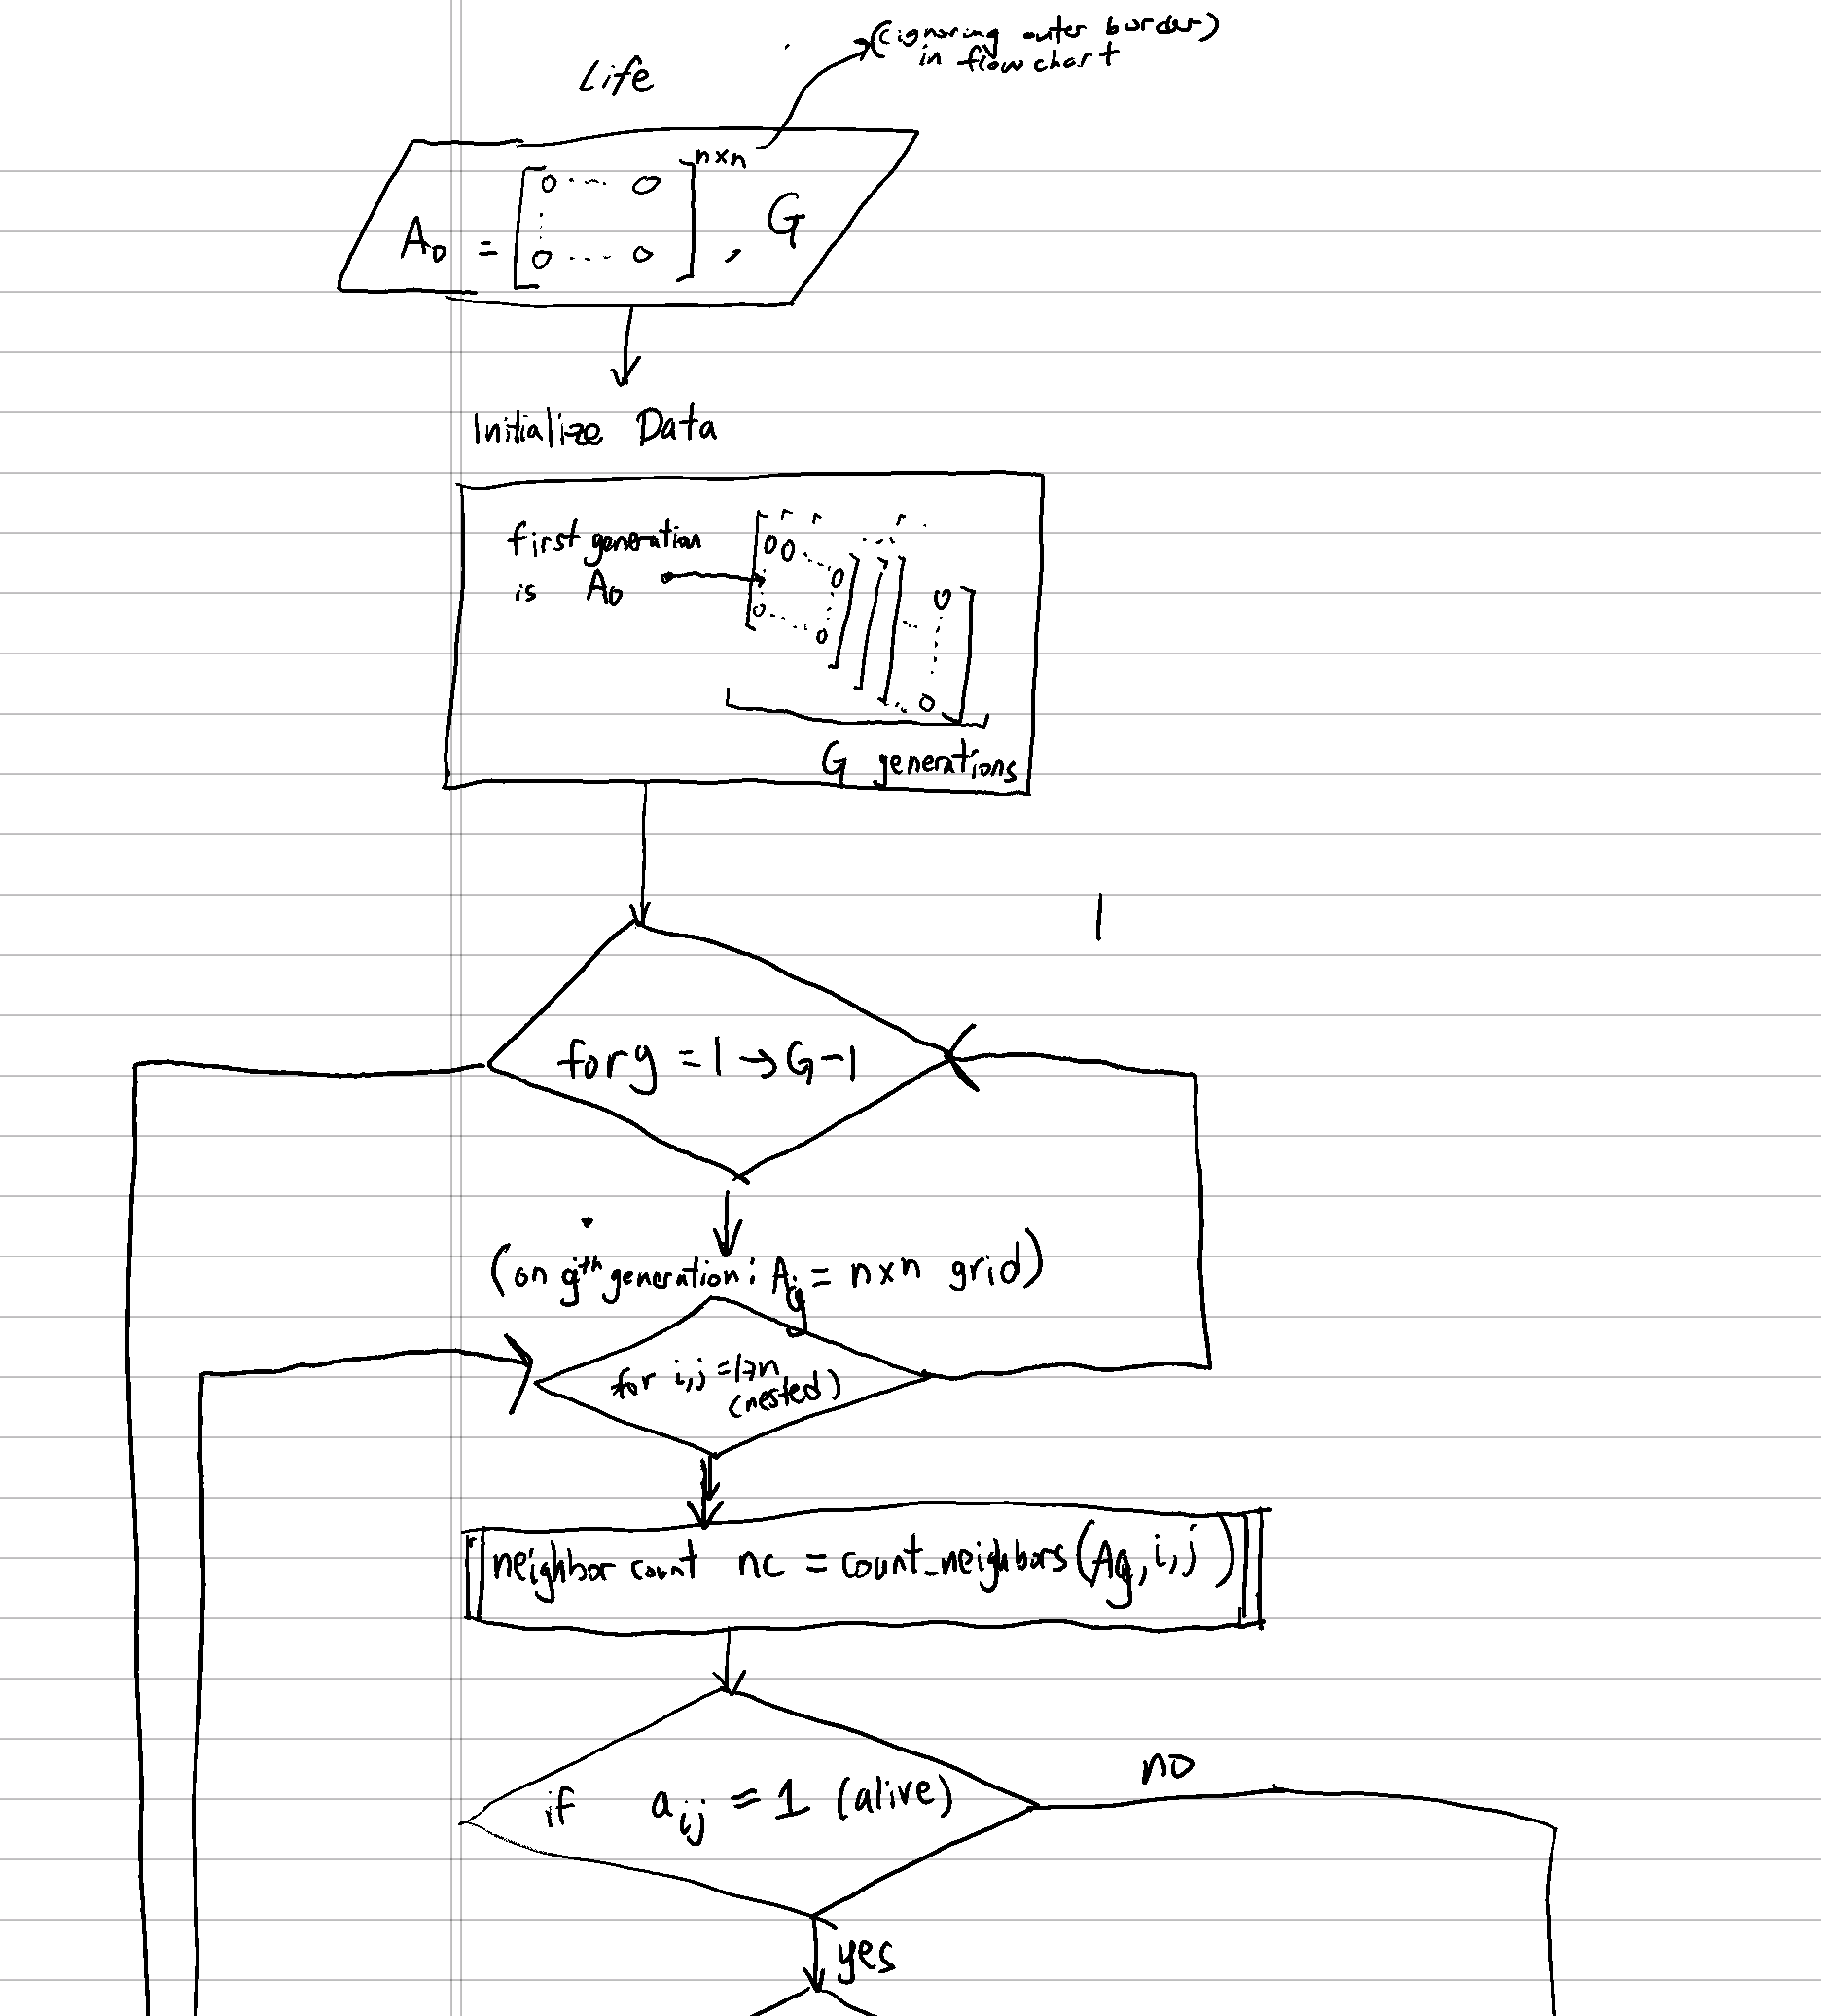
\includegraphics[scale=0.2]{pseudocode1a.png}

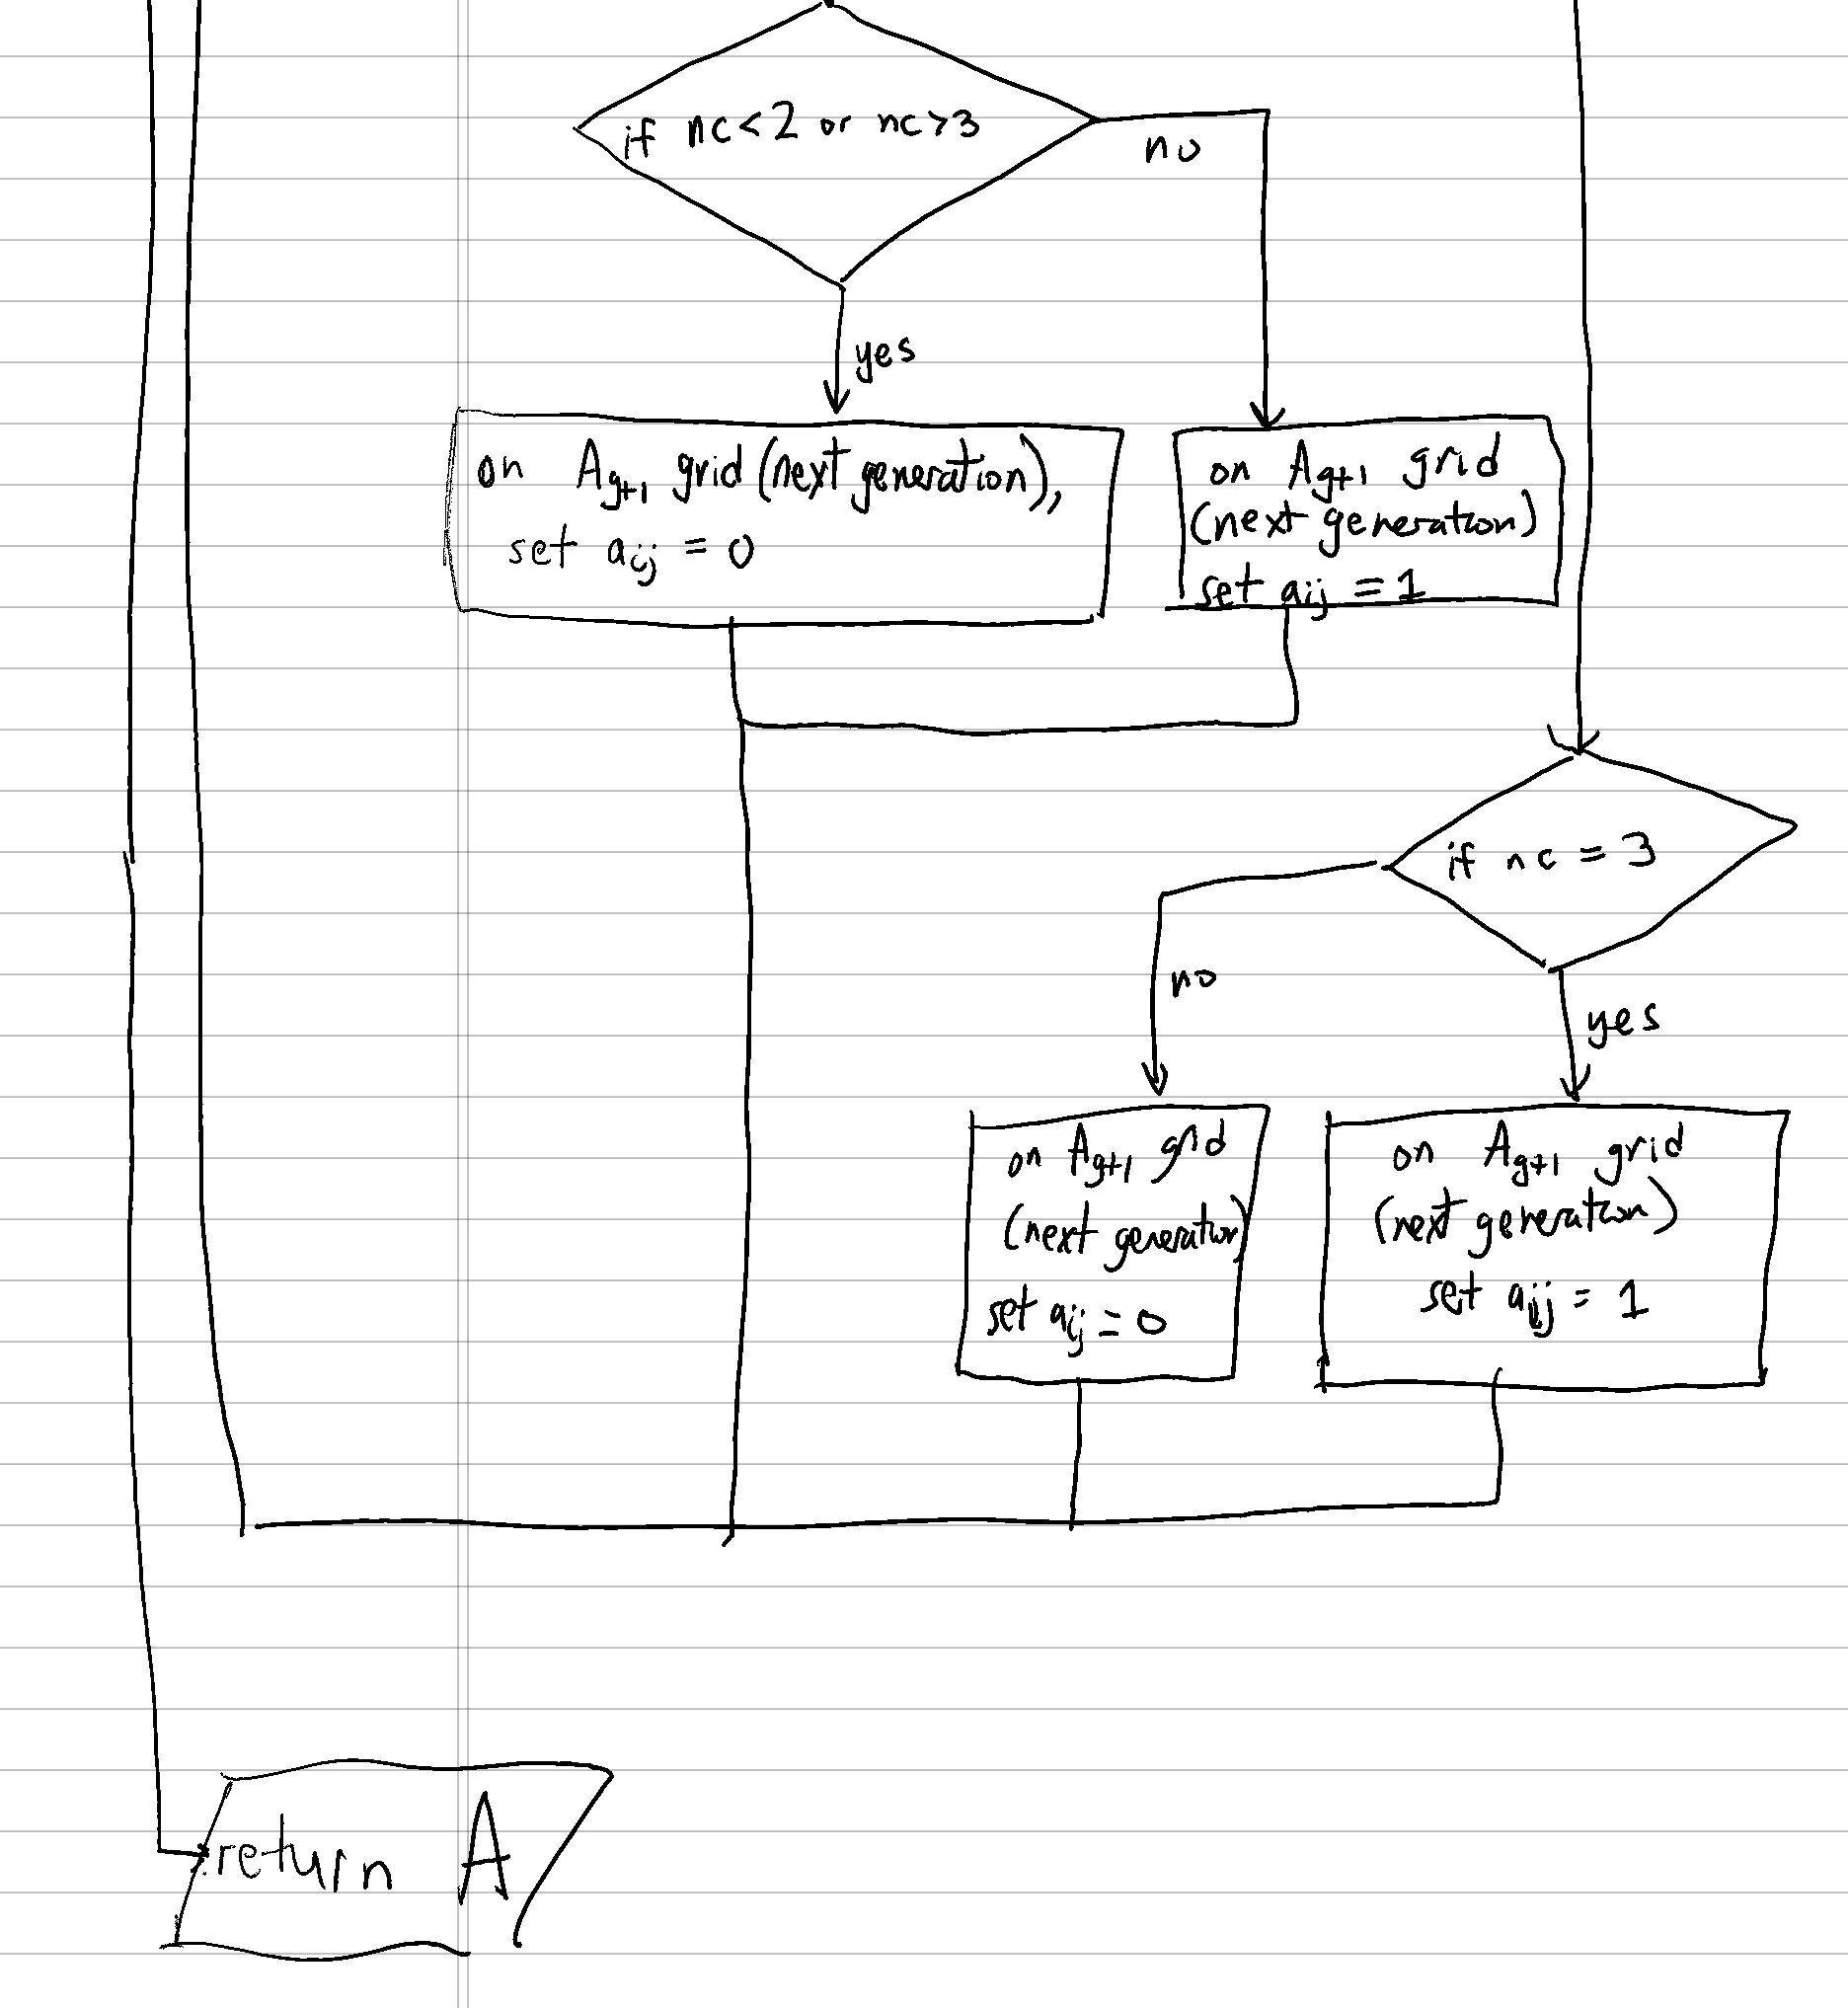
\includegraphics[scale=0.2]{pseudocode1b.png}

\pagebreak
Counting Neighbors

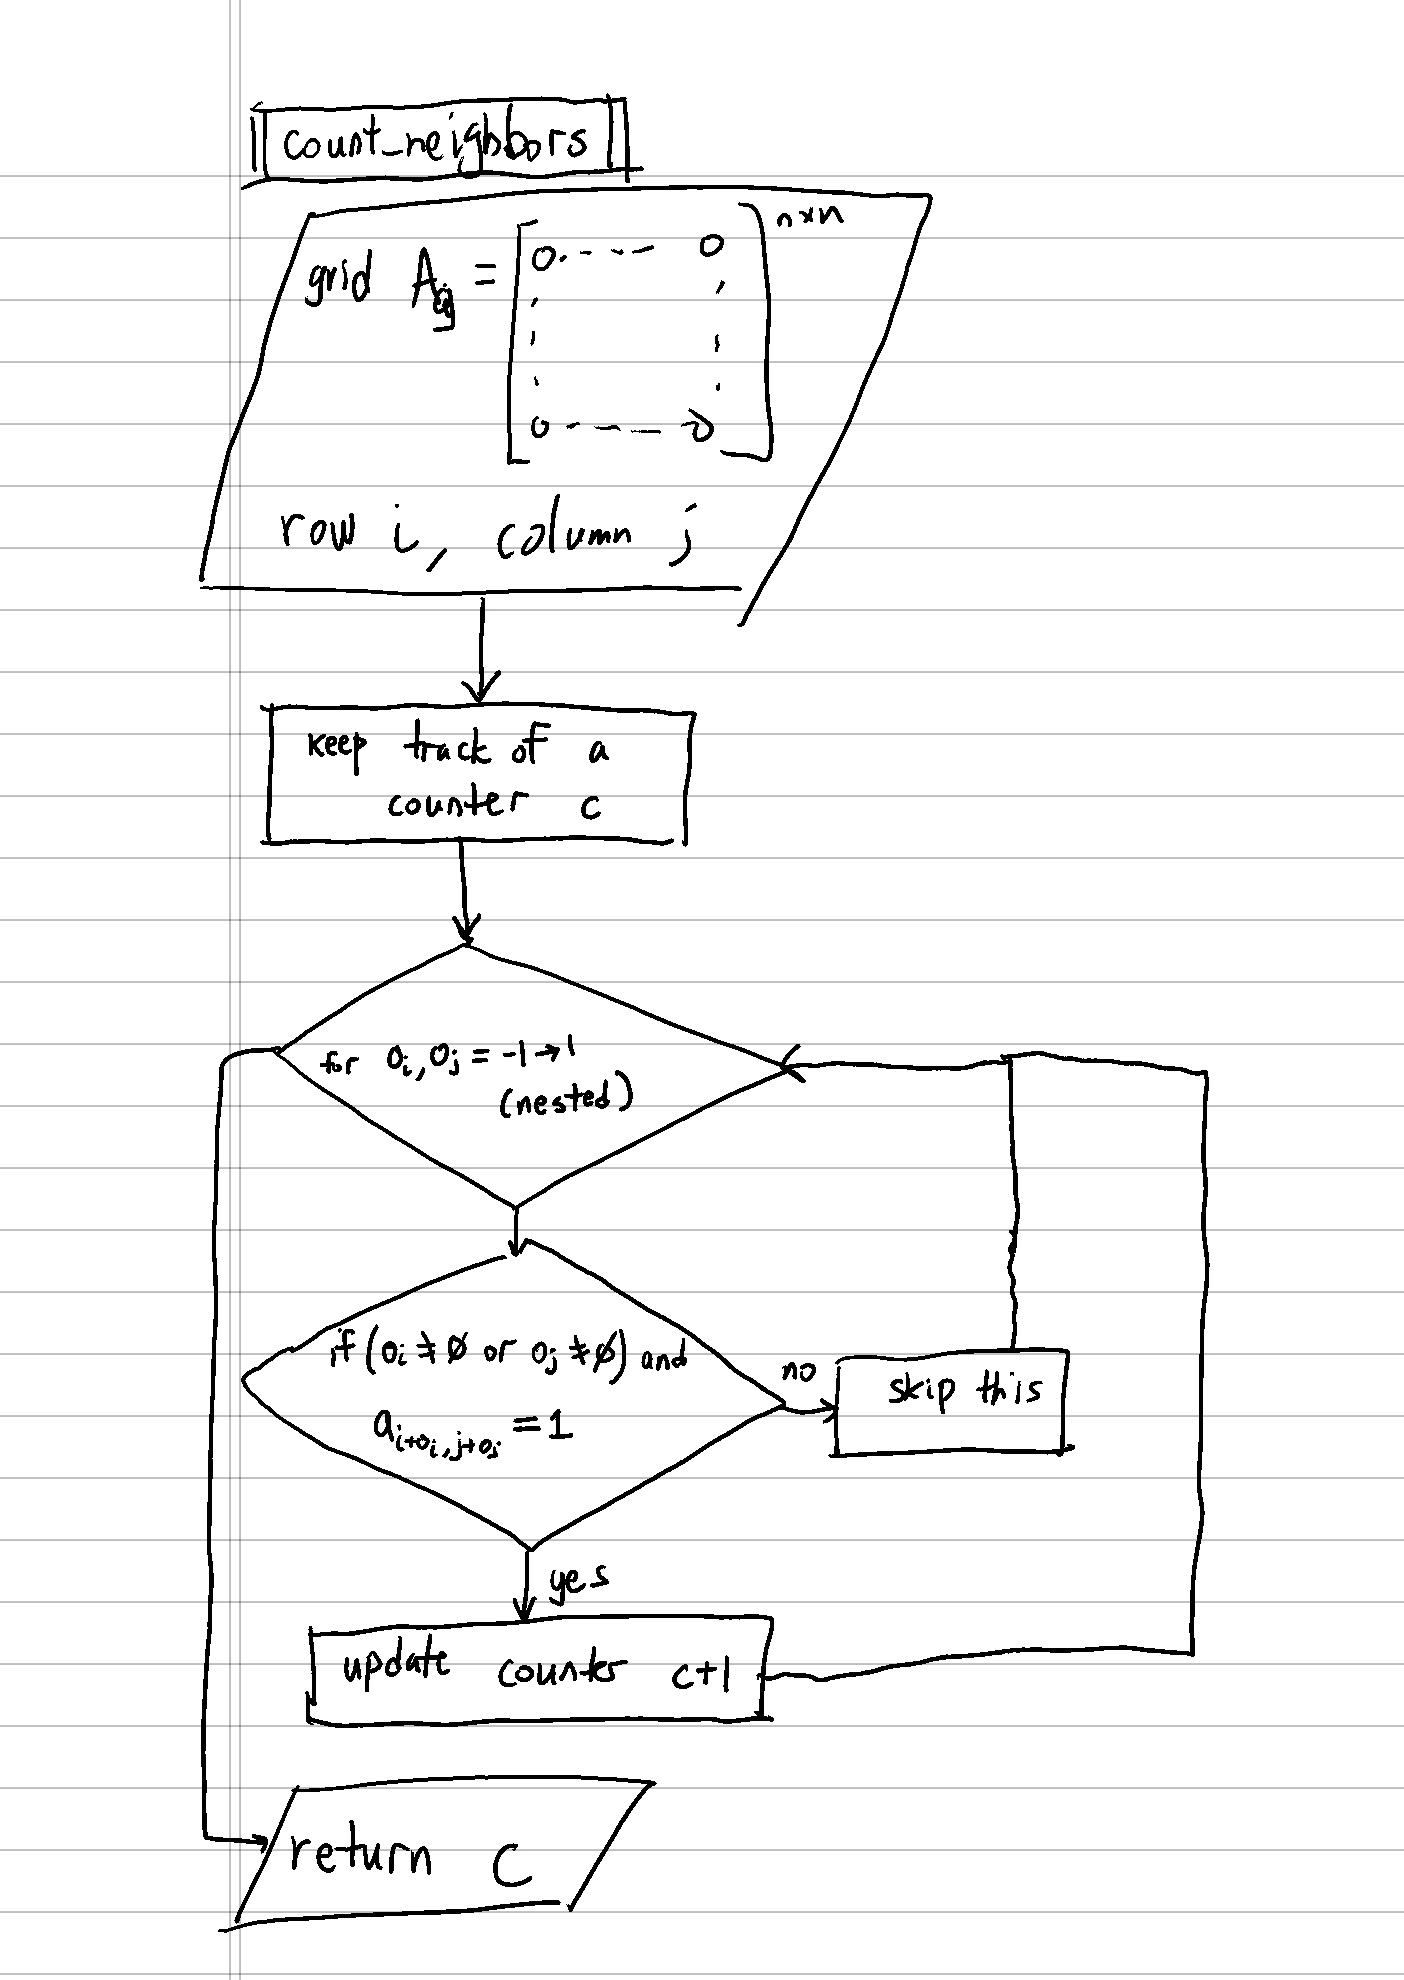
\includegraphics[scale=0.25]{pseudocode2.png}
\pagebreak

\section{Code}

Life.m

\begin{verbatim}
%   A Function that Simulates the Game of Life
%
% Input:
%
%   Init_Config: An nxn matrix of cells containing either a 1 (alive) or 0
% (dead). Acts as the initial configuration of the grid and is the first
% one on the series of grids.
%
%   Generations: An integer containing the number of "frames" this
% simulation plays through. 
%
% Output:
%
%   Simulation: A 3-dimensional matrix containing Generations "frames" of
% nxn grids (nxnxGenerations) of the Game of Life being simulated on each
% "frame"
function [Simulation] = Life(Init_Config, Generations)
    n = size(Init_Config, 1);
    A = zeros(n+2, n+2, Generations);
    
    % initializing the first generation to Init_Config
    for i=1:n
        for j=1:n
            A(i+1, j+1, 1) = Init_Config(i, j);
        end
    end

    % the first generation is already set so we only need
    % to set after the first one
    for g=1:Generations-1
        % A_g is the gth generation of A
        A_g = A(:,:,g);

        % need to check (2, n+1) instead of (1, n)
        % because A has a "border" of zeros so we
        % really need to access indices 2-(n+1)
        for i=2:n+1
            for j=2:n+1
                nc = count_neighbors(A_g, i, j);
                if A_g(i, j) == 1
                    if nc < 2 || nc > 3
                        A(i, j, g+1) = 0;
                    else
                        A(i, j,g+1) = 1;
                    end
                else
                    if nc == 3
                        A(i, j, g+1) = 1;
                    else
                        A(i, j, g+1) = 0;
                    end
                end

            end
        end
    end

    % return
    Simulation = A;

end 
\end{verbatim}

counting\_neighbors.m

\begin{verbatim}
% A function that counts the "neighboring cells" of (i, j) by using a
% nested for loop
% 
% Input:
%
%   A_g: A (n+1)x(n+1) matrix that contains the gth "frame" of the
% simulation in Life
%
%   i, j: The coordinates (row, col) of A_g that we want to cout the
% neighboring cells of
function [c] = count_neighbors(A_g, i, j)
    c = 0;

    % for looping through the "offsets":
    % : (-1, -1), (-1, 0), ..., (1, 1)
    % such that for each offset o = (oi, oj) 
    % (where i is row and j is column)
    % we can count the neighboring cell of (i, j) with
    % (i + oi, j + oj)
    for oi = -1:1
        for oj = -1:1
            % counting if neighboring cell is alive
            if (oi ~= 0 || oj ~= 0) && A_g(i+oi, j+oj) == 1
                c = c + 1;
            end
        end
    end
    
    % return (c is already c :P)

end
\end{verbatim}
\pagebreak

\section{Some proof it works}

Unfortunately, this doesn't work as well in pdf form, so the gifs are provided in the 
zip. But the Doc is on the next page. 

\end{document}